\documentclass[12pt,a4paper]{article}
\usepackage{cmap} % Makes the PDF copiable. See http://tex.stackexchange.com/a/64198/25761
\usepackage[T1]{fontenc}
\usepackage[brazil]{babel}
\usepackage[utf8]{inputenc}
\usepackage{amsmath}
\usepackage{amsfonts}
\usepackage{amssymb}
\usepackage{amsthm}
\usepackage[usenames,svgnames,dvipsnames]{xcolor}
\usepackage{hyperref}
\usepackage{multicol}
\usepackage{graphicx}
\usepackage[margin=2cm]{geometry}

\hypersetup{
    colorlinks = true,
    allcolors = {blue}
}

% TODO: Consider using exsheets
% http://linorg.usp.br/CTAN/macros/latex/contrib/exsheets/exsheets_en.pdf
%
% http://ctan.org/tex-archive/macros/latex/contrib/exercise/
% Options: answerdelayed,lastexercise,noanswer
\usepackage[answerdelayed,lastexercise]{exercise}

\addto\captionsbrazil{%
\def\listexercisename{Lista de exerc\'icios}%
\def\ExerciseName{Exerc\'icio}%
\def\AnswerName{Solu\c{c}\~ao do exerc\'icio}%
\def\ExerciseListName{Ex.}%
\def\AnswerListName{Solu\c{c}\~ao}%
\def\ExePartName{Parte}%
\def\ArticleOf{de\ }%
}

\renewcommand{\ExerciseHeaderTitle}{(\ExerciseTitle)\ }
\renewcommand{\ExerciseListHeader}{%\ExerciseHeaderDifficulty%
\textbf{%\ExerciseListName\
\ExerciseHeaderNB.\ %
%\ --- \
\ExerciseHeaderTitle}%
%\ExerciseHeaderOrigin
\ignorespaces}
\renewcommand{\AnswerListHeader}{\textbf{\ExerciseHeaderNB.\ (\AnswerListName)\ }}

\newtheorem*{note}{Observação}
\newcommand*\diff{\mathop{}\!\mathrm{d}}
\newcommand*\sen{\operatorname{sen}}

\renewcommand{\theenumi}{\alph{enumi}}
\renewcommand\labelenumi{(\theenumi) }

\newcommand*\tipo{Prova I}
\newcommand*\turma{NEXM241-A}
\newcommand*\disciplina{CDI2001}
\newcommand*\eu{Helder G. G. de Lima}
\newcommand*\data{06/04/2024}

\author{\eu}
\title{\tipo - \disciplina}
\date{\data}

\begin{document}
\thispagestyle{empty}
\newgeometry{margin=2cm,bottom=0.5cm}
\begin{center}

\includegraphics[width=9.0cm]{marca} \\
\textbf{\tipo\ (\disciplina / \turma)} \\
Prof. \eu\footnote{
Este é um material de acesso livre distribuído sob os termos da licença \href{https://creativecommons.org/licenses/by-sa/4.0/deed.pt_BR}{Creative Commons BY-SA 4.0}}
\end{center}

\noindent Nome do(a) aluno(a): \underline{\hspace{9,7cm}} Data: \underline{\data}

%\section*{Instruções}
\begin{center}\fbox{
\begin{minipage}{14cm}

{\footnotesize
\begin{itemize}
\renewcommand{\theenumi}{\Roman{enumi}}
\item Identifique-se em todas as folhas.
\item Mantenha o celular e os demais equipamentos eletrônicos desligados durante a prova.
\item Justifique cada resposta com cálculos ou argumentos baseados na teoria estudada.
\item Resolva $5$ das $6$ questões (deixe claro que questão não deverá ser corrigida).
\end{itemize}
}

\end{minipage}
}
\end{center}

%\section*{Questões}
\begin{ExerciseList}


\Exercise[title={2,0}]
Considere a função integrável $f:[-2, 0] \to [0,4]$ dada por $f(x)=4-x^2$. Utilize um limite de somas superiores para calcular a integral definida $\int_{-2}^0 f(x) \diff{x}$.

Lembrete:
\(
  1 + 2 + \cdots + n = \frac{n(n+1)}{2}
\)
e
\(
  1^2 + 2^2 + \cdots + n^2 = \frac{n(n+1)(2n+1)}{6}
\)
.
\Answer A resolução consistirá das seguintes etapas:
\begin{itemize}
  \item Obter uma partição do intervalo $[-2, 0]$ com $n$ subintervalos de mesmo comprimento
  \item Identificar em que extremidade de cada intervalo a função assume seu valor máximo (pois devem ser usadas somas superiores)
  \item Expressar a soma superior correspondente à partição obtida em termos de $n$
  \item Obter a integral como um limite da soma superior quando $n$ tende a infinito
\end{itemize}

Seja $P = \{ x_0, \ldots, x_n \}$ a partição do intervalo $[-2, 0]$ em $n$ subintervalos de mesmo comprimento $\Delta x = \frac{2}{n}$, isto é,
\[
  x_0 = -2,\quad
  x_1 = -2 + \Delta x,\quad
  x_2 = -2 + 2\Delta x,\quad
  \quad\ldots,\quad
  x_n = -2 + n\Delta x = 0.
\]

Como $f$ é uma função crescente (pois sua derivada $f^\prime(x) = -2x > 0$ para $x \in [-2, 0]$), o valor máximo de $f$ em cada subintervalo $[x_{i-1}, x_i]$ é alcançado na extremidade direita, $x_i$. A figura a seguir mostra o caso em que $n = 6$:

\begin{center}
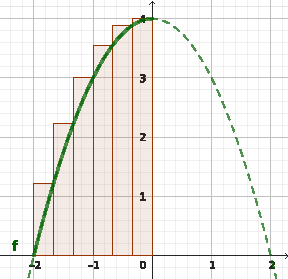
\includegraphics[width=5.0cm]{img/prova-1-nex-soma-superior.pdf}
\end{center}

Deste modo, a soma superior correspondente à partição $P$ é:
\begin{align*}
  \overline{S}(f, P)
  & = \sum_{i=1}^n f(x_i) \Delta x
    = \sum_{i=1}^n \left(4-x_i^2\right) \Delta x
    = \sum_{i=1}^n \left(4-(-2 + i\Delta x)^2\right) \Delta x \\
  & = \sum_{i=1}^n \left(4-(4 - 4i\Delta x + i^2(\Delta x) ^2)\right) \Delta x
    = \sum_{i=1}^n \left(4i\Delta x - i^2(\Delta x) ^2\right) \Delta x \\
  & = \sum_{i=1}^n 4i(\Delta x)^2 - i^2(\Delta x)^3
    = \sum_{i=1}^n 4i\left(\frac{2}{n}\right)^2 - i^2\left(\frac{2}{n}\right)^3
    = 4 \left(\frac{2}{n}\right)^2 \sum_{i=1}^n i - \left(\frac{2}{n}\right)^3\sum_{i=1}^n i^2 \\
  & = \frac{16}{n^2} \left(\frac{(1+n)n}{2}\right) - \frac{8}{n^3}\left(\frac{n(n+1)(2n+1)}{6}\right)
    = \frac{16}{3} + \frac{4}{n} - \frac{4}{3n^2}.
\end{align*}
Logo, $\int_{-2}^0 4-x^2\diff{x} = \lim_{n \to \infty} \frac{16}{3} + \frac{4}{n} - \frac{4}{3n^2} = \frac{16}{3} \approx 5,3333$.

\begin{note}
  Pode-se validar a resposta obtida calculando a mesma integral por meio do teorema fundamental do cálculo:
  \[
    \int_{-2}^0 4-x^2\diff{x}
    = \left(4x-\frac{x^3}{3}\right)\bigg\rvert_{-2}^0
    = \left(0-\frac{0}{3}\right) - \left(-8-\frac{-8}{3}\right)
    = \frac{16}{3}.
  \]
\end{note}


\Exercise[title={2,0}]
Calcule a integral definida $\int_{\frac{\pi}{6}}^{\frac{5\pi}{6}} x\cos(x) \diff{x}$.
\Answer Pode-se aplicar integração por partes considerando
\begin{align*}
  u=x
  & \Rightarrow \diff{u} = \diff{x}, \text{ e} \\
  \diff{v} = \cos(x) \diff{x},
  & \Rightarrow v = \int \cos(x) \diff{x} = \sen(x).
\end{align*}
Neste caso, considerando o intervalo de integração dado, tem-se:
\begin{align*}
  \int_{\frac{\pi}{6}}^{\frac{5\pi}{6}} x\cos(x) \diff{x}
  & = \left(x \sen(x) \right)\bigg\rvert_{\frac{\pi}{6}}^{\frac{5\pi}{6}}
    - \int_{\frac{\pi}{6}}^{\frac{5\pi}{6}} \sen(x) \diff{x}
    = \left(x \sen(x) \right)\bigg\rvert_{\frac{\pi}{6}}^{\frac{5\pi}{6}}
    + \cos(x) \bigg\rvert_{\frac{\pi}{6}}^{\frac{5\pi}{6}} \\
  & = \left(\frac{5\pi}{6}\sen\left(\frac{5\pi}{6}\right) - \frac{\pi}{6}\sen\left(\frac{\pi}{6}\right)\right) + \left(\cos\left(\frac{5\pi}{6}\right)-\cos\left(\frac{\pi}{6}\right)\right) \\
  & = \left(\frac{5\pi}{6}\cdot \frac{1}{2} - \frac{\pi}{6}\cdot \frac{1}{2}\right) + \left(-\frac{\sqrt{3}}{2}-\frac{\sqrt{3}}{2}\right)
    = \frac{\pi}{3} - \sqrt{3}
    \approx -0,6849.
\end{align*}

\textbf{Solução 2}: Também é possível aplicar a integração por partes à integral indefinida, obtendo $\int x\cos(x) \diff{x} = x\sen(x) +\cos(x) + C$ e então aplicar o teorema fundamental do cálculo para calcular a integral definida correspondente ao intervalo dado, obtendo o mesmo valor final.

\begin{note}
Para validar a resposta, pode-se calcular a derivada da primitiva obtida, para comprovar que é igual a $x \cos(x)$. Além disso, pode-se esboçar o gráfico de $f(x) = x \cos(x)$ e observar que a maior parte da área entre o gráfico e o eixo $x$ está abaixo do eixo, indicando que a integral definida deve ser negativa:

\begin{center}
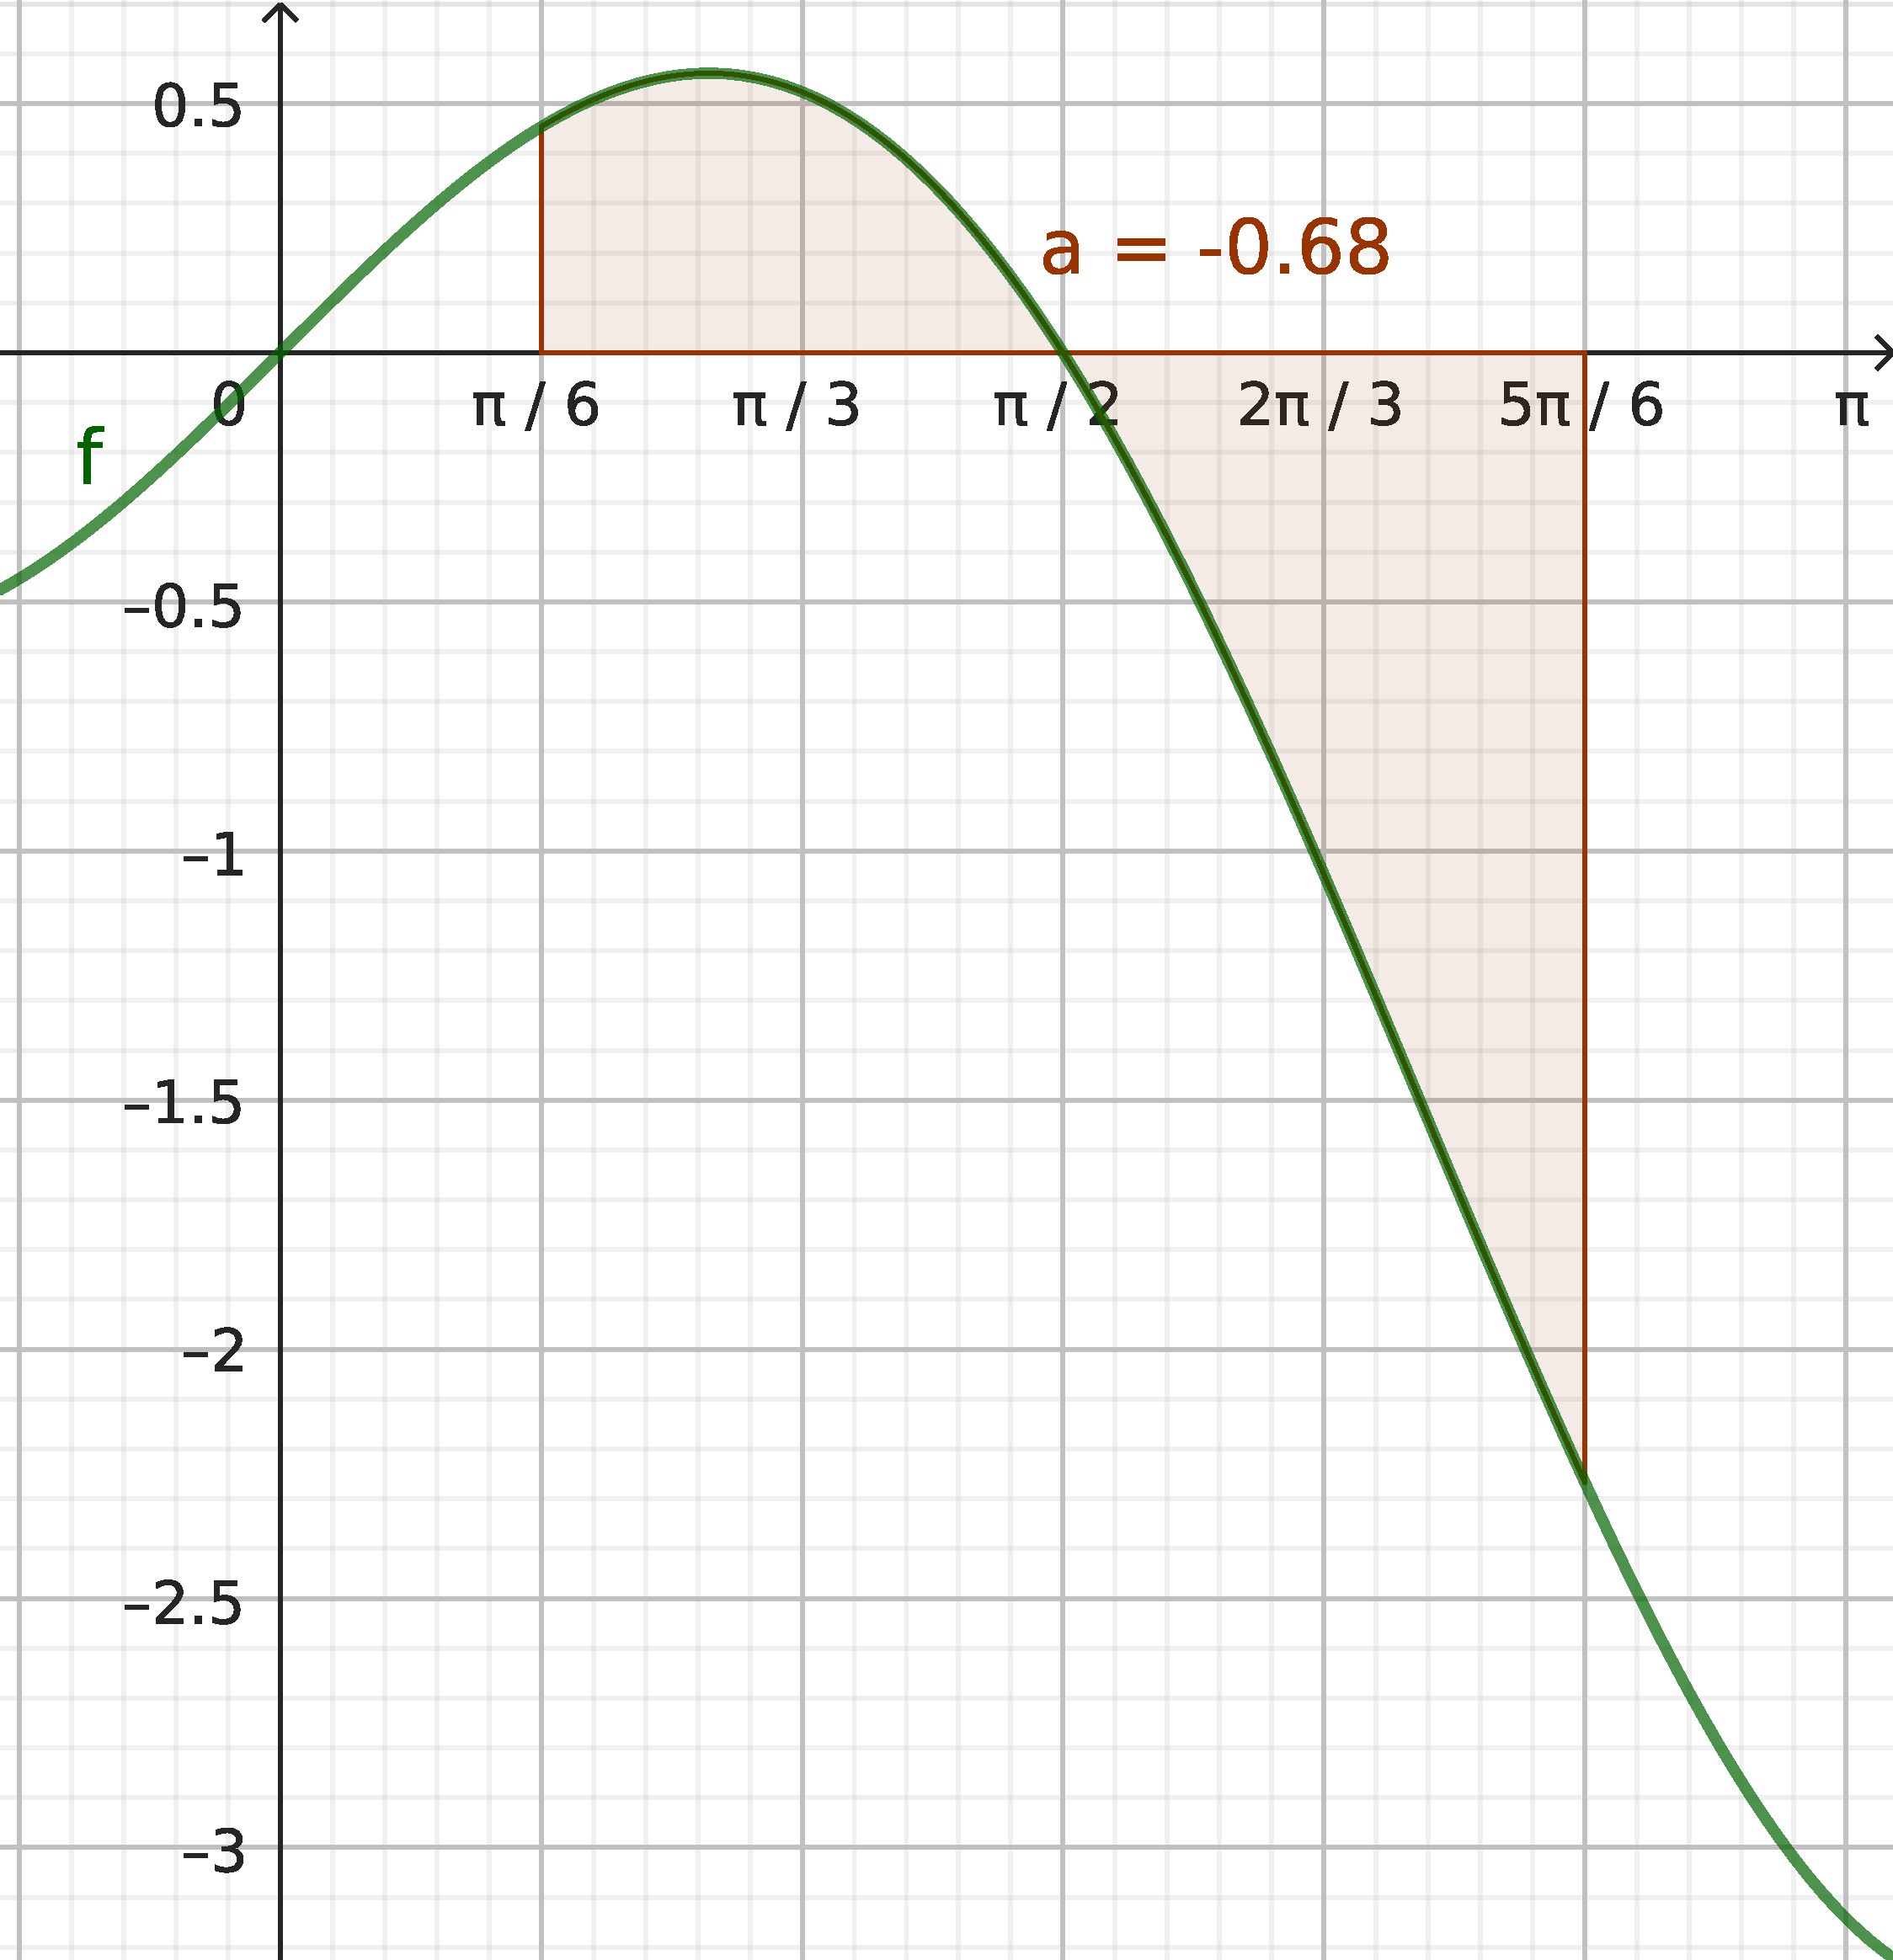
\includegraphics[width=6.0cm]{img/prova-1-nex-integral-por-partes.pdf}
\end{center}
\end{note}

\Exercise[title={2,0}]
Determine se a integral $\int_0^{1/\pi} \frac{1}{x^2} \cos\left(\frac{1}{x}\right) \diff{x}$ é convergente ou divergente.
\Answer Note que o domínio da função $f(x) = \frac{1}{x^2} \cos\left(\frac{1}{x}\right)$ é $D_f = (-\infty, 0) \cup (0, \infty)$. Logo, a extremidade à esquerda do intervalo de integração não está no domínio de $f$. Por definição, a convergência da integral imprópria dada equivale à existência de um limite de integrais definidas:
\[
I
= \int_0^{1/\pi} \frac{1}{x^2} \cos\left(\frac{1}{x}\right) \diff{x}
= \lim_{a\to 0^+} \int_a^{1/\pi} x^{-2} \cos\left(\frac{1}{x}\right) \diff{x}.
\]
Fazendo a mudança de variável $u = \frac{1}{x}$, tem-se $\diff{u} = -x^{-2}\diff{x}$. Além disso, para $x = a > 0$, tem-se $u = \frac{1}{a}$ e para $x = \frac{1}{\pi}$, tem-se $u = \pi$. Logo,
\begin{align*}
  \int_a^{1/\pi} x^{-2} \cos\left(\frac{1}{x}\right) \diff{x}
  & = \int_{\frac{1}{a}}^{\pi} - \cos\left(u\right) \diff{u}
    = - \int_{\frac{1}{a}}^{\pi} \cos\left(u\right) \diff{u} \\
  & = - \left(\sen{u} \right)\bigg\rvert_{\frac{1}{a}}^{\pi}
    = - \left(\sen(\pi) - \sen\left(\frac{1}{a}\right)\right)
    = \sen\left(\frac{1}{a}\right).
\end{align*}

Assim, a integral é divergente, pois $\displaystyle I = \lim_{a\to 0+} \sen\left(\frac{1}{a}\right)$ equivale a $\displaystyle I = \lim_{u\to +\infty} \sen(u)$, que não existe, já que $\sen(u) = 0$ sempre que $u = k \pi$ e $\sen(u) = 1$ sempre que $u = \frac{\pi}{2} + 2 k \pi$, $k \in \mathbb{Z}$.


\Exercise[title={2,0}] Determine a área da região do primeiro quadrante, delimitada pelos gráficos das funções $f(x)=\dfrac{12}{x + 1}$ e $g(x)=7-x$ e pelos eixos coordenados.
\Answer Observe que o gráfico de $f$ é uma hipérbole e o de $g$ é uma reta. Essas curvas se intersectam quando $f(x) = g(x)$, isto é,
\[
  \dfrac{12}{x + 1} = 7-x
  \Leftrightarrow 12 = (7 - x) \cdot (x + 1)
  \Leftrightarrow 12 = -x^2 + 6x +7
  \Leftrightarrow x^2 - 6x + 5 = 0
  \Leftrightarrow (x - 1) \cdot(x - 5) = 0.
\]
Logo, há dois pontos de interseção: $P_1 = (1, g(1)) = (1, 6)$ e $P_2 = (5, g(5)) = (5, 2)$. A figura a seguir mostra a região de interesse:

\begin{center}
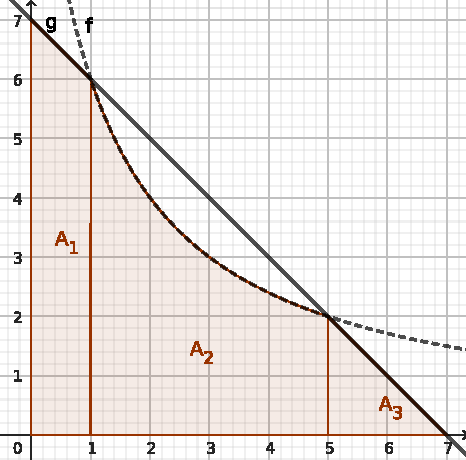
\includegraphics[width=6.0cm]{img/prova-1-nex-afim-racional-e-eixos.pdf}
\end{center}

Conforme indicado, o gráfico de $f$ está abaixo do de $g$ entre os pontos de intersecção, e acima do de $g$ no restante do intervalo. Então, a área da região é a soma de três integrais, $A = A_1 + A_2 + A_3$, em que:
\begin{align*}
  A_1 & = \int_0^1 7 - x \diff{x}
      = \left( 7x - \frac{x^2}{2} \right)\bigg\rvert_0^1
      = \left( \frac{14x - x^2}{2} \right)\bigg\rvert_0^1
      = \frac{14-1}{2} - \frac{0}{2}
      = \frac{13}{2} \text{ u.a.}\\
  A_2 & = \int_1^5 \frac{12}{x + 1} \diff{x}
        = 12 \int_1^5 \frac{1}{x + 1} \diff{x}
        = 12 \int_2^6 \frac{1}{u} \diff{u}
        = 12 \ln(u)\big\rvert_2^6
        = 12 (\ln(6) - \ln(2)) \\
      & = 12 \ln(3) \text{ u.a.}\\
  A_3 & = \int_5^7 7 - x \diff{x}
      = \left( \frac{14x - x^2}{2} \right)\bigg\rvert_5^7
      = \frac{14\cdot 7 - 7^2}{2} - \frac{14\cdot 5 - 5^2}{2}
      = \frac{49}{2} - \frac{45}{2}
      = 2 \text{ u.a.}.
\end{align*}

Portanto, $A = \frac{13}{2} + 12 \ln(3) + 2 = \frac{17}{2} + 12\ln(3) \approx 21,68$ u. a..

\begin{note}
  Para fins de validação da resposta, observe que a região é ``um pouco menor'' que a metade do quadrado $[0, 7] \times [0, 7]$. Logo, o resultado obtido está coerente, pois é ``um pouco menor'' do que a metade da área do quadrado, que é $\frac{49}{2} = 24,5 \text{ u.a.}$.
\end{note}


\Exercise[title={2,0}]
Calcule a área da região simultaneamente interior ao limaçon \(r = 2 + \sen(\theta)\) e exterior ao limaçon \(r = 2 - \sen(\theta)\):

\includegraphics[width=7.0cm]{img/prova-1-nex-limaçons.pdf}

\Answer A área da região hachurada é a diferença entre a área da região interior ao limaçon \(r = 2 + \sen(\theta)\) e a área interior ao limaçon \(r = 2 - \sen(\theta)\). Além disso, cada um dos pontos \((r, \theta)\) da região tem ângulo
$\theta \in [0, \pi]$ e raio $r \in [2 - \sen(\theta), 2 + \sen(\theta)]$. Logo, a área $A$ da região é dada por
\begin{align*}
  A
  & = \frac{1}{2}\int_0^\pi \left(2 + \sen(\theta)\right)^2 \diff\theta
      -
      \frac{1}{2}\int_0^\pi \left(2 - \sen(\theta)\right)^2 \diff\theta \\
  & = \frac{1}{2}\int_0^\pi \left(2 + \sen(\theta)\right)^2 - \left(2 - \sen(\theta)\right)^2 \diff\theta \\
  & = \frac{1}{2}\int_0^\pi \left(4 + 4\sen(\theta) + \sen^2(\theta)\right) - \left(4 - 4\sen(\theta) + \sen^2(\theta)\right) \diff\theta \\
  & = \frac{1}{2}\int_0^\pi 8\sen(\theta) \diff\theta
    = \frac{8}{2}\int_0^\pi \sen(\theta) \diff\theta \\
  & = 4 \cdot \left( -\cos(\theta) \right)\big\rvert_0^\pi
    = 4 \cdot \left( -\cos(\pi) - (-\cos(0))\right)
    = 4 \cdot \left(-(-1) + 1 \right)
    = 8 \text{ u.a.}.
\end{align*}


\Exercise[title={2,0}]
Calcule o comprimento de arco da função $f(x) = e^x + \frac{1}{4}e^{-x}$ entre $x=-1$ e $x=1$.
\Answer A figura a seguir mostra o gráfico de $f$ no intervalo de interesse:

\begin{center}
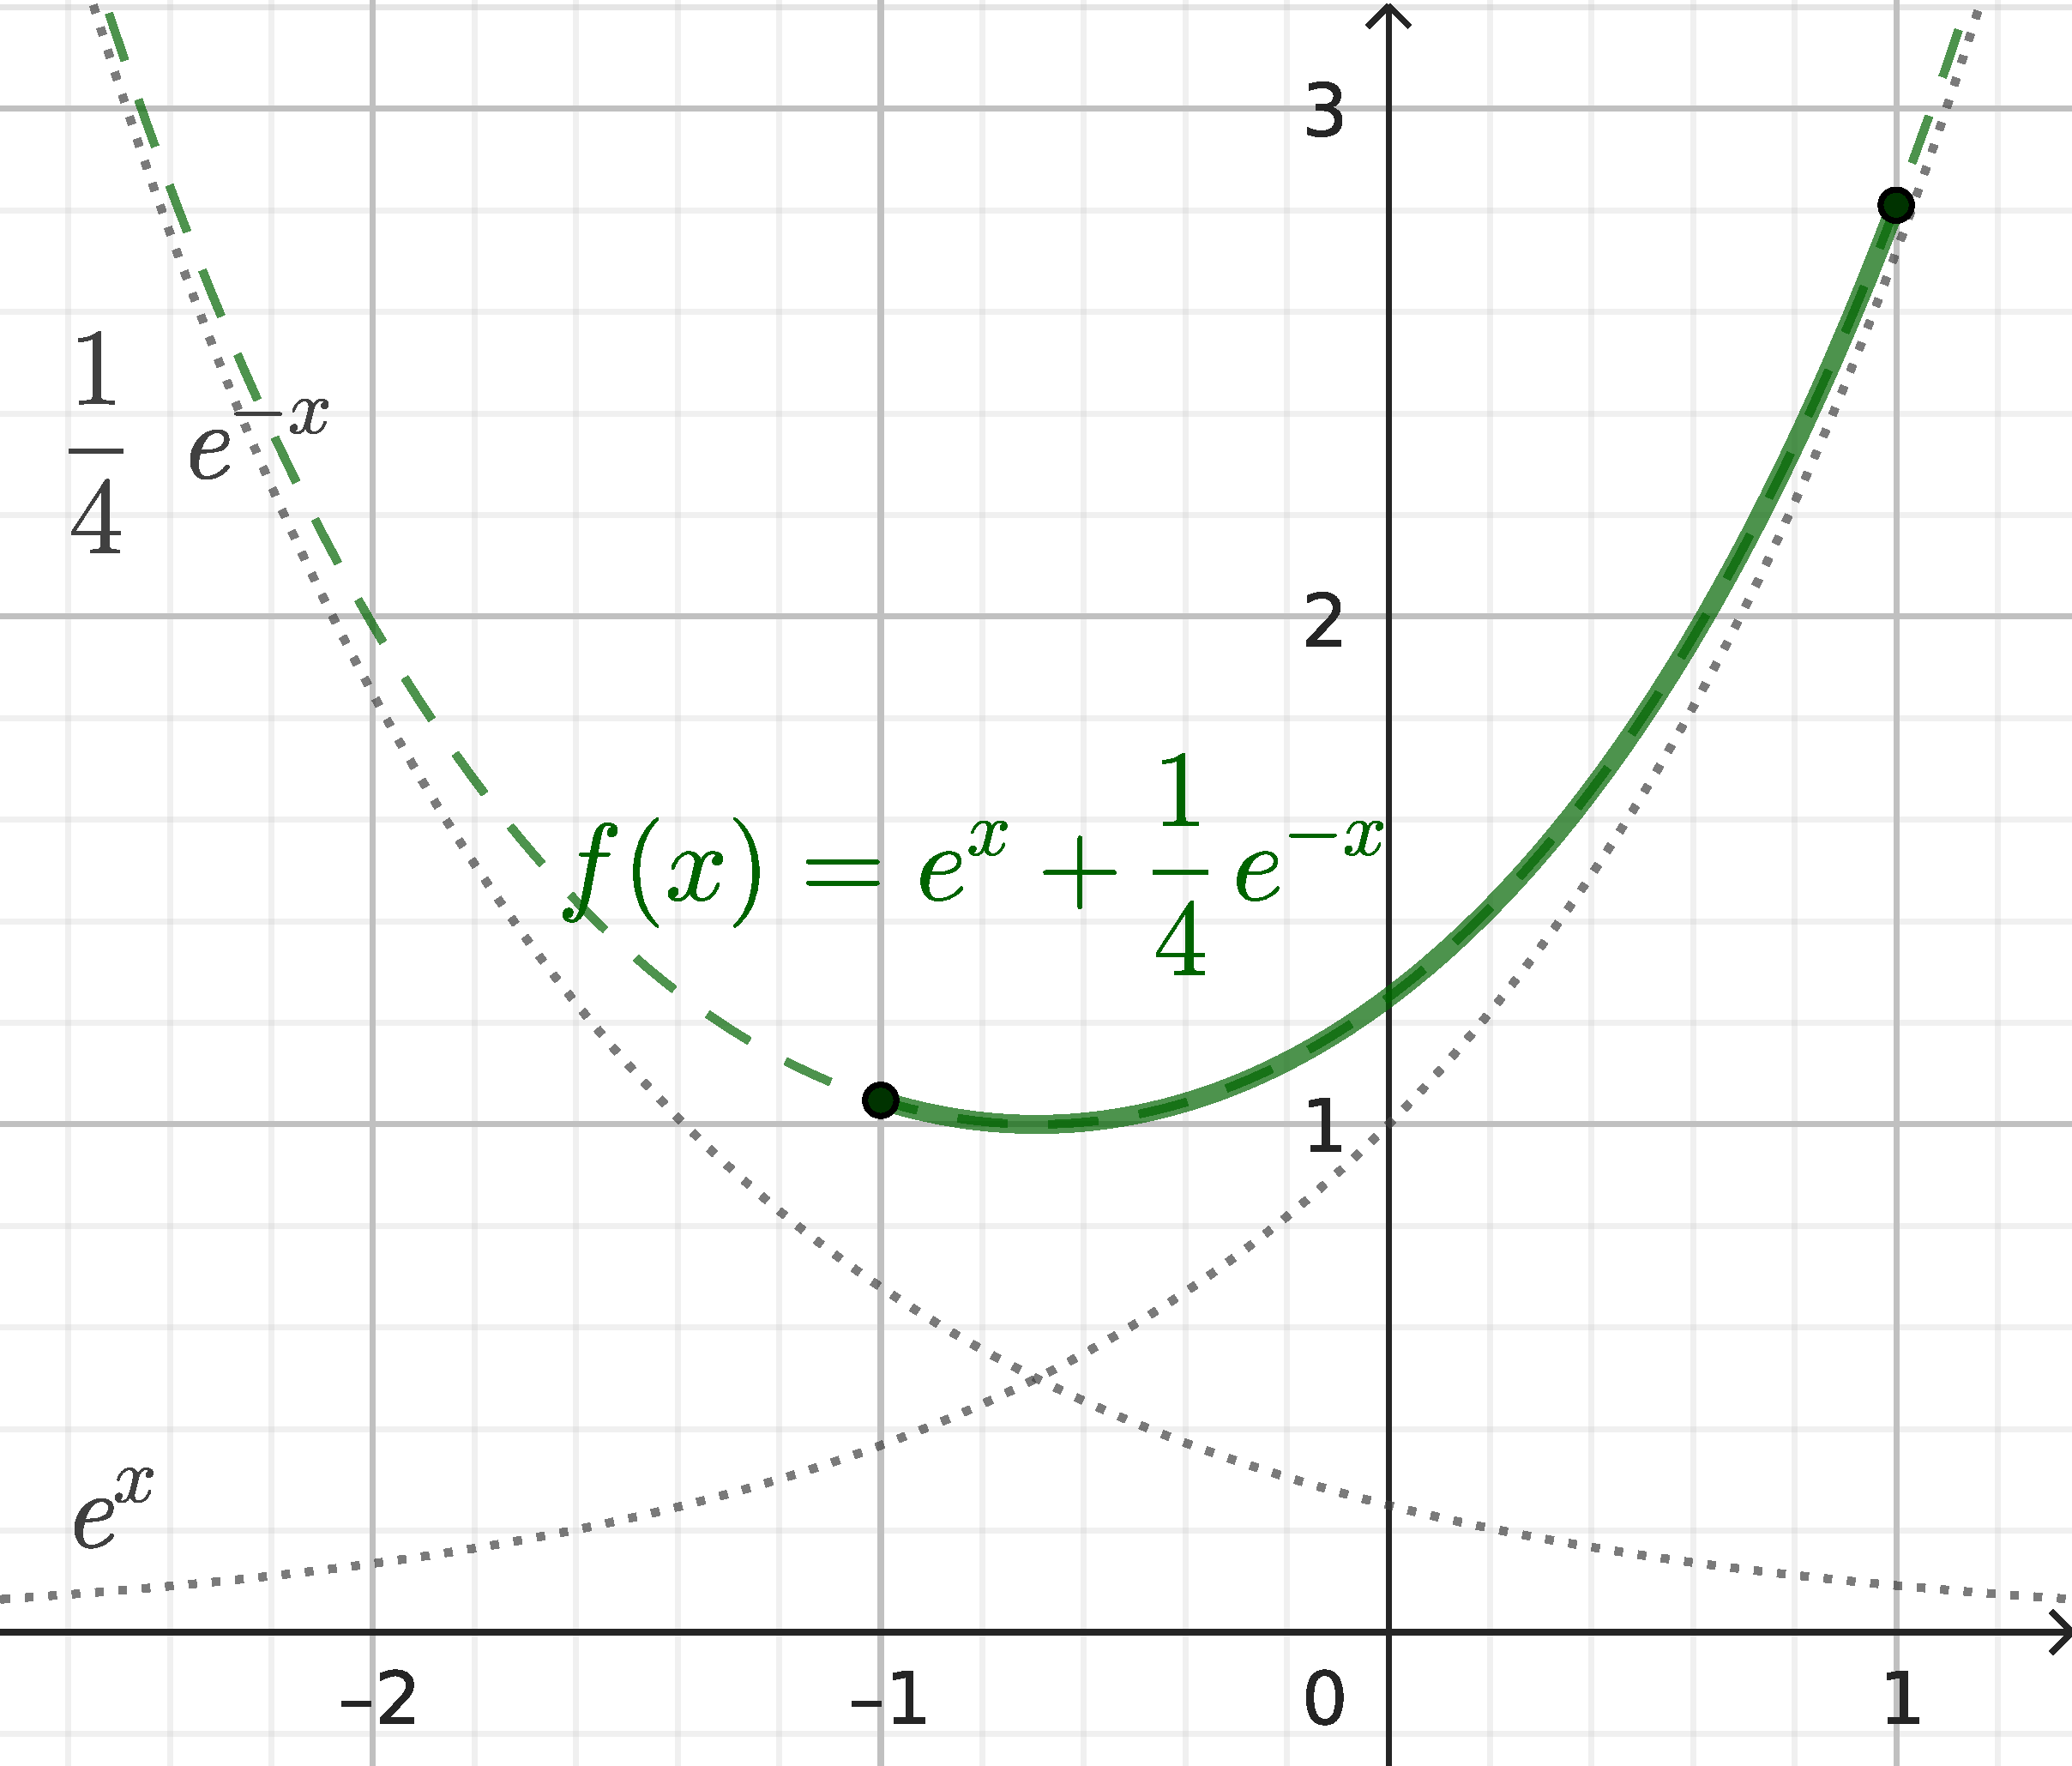
\includegraphics[width=6.0cm]{img/prova-1-nex-comprimento-de-arco.pdf}
\end{center}

O comprimento de arco é dado por $L = \int_{-1}^1 \sqrt{1 + \left(f^\prime(x)\right)^2} \diff{x}$, em que:
\[
  f^\prime(x)
  = \left(e^x + \frac{1}{4} e^{-x}\right)^\prime
  = e^x - \frac{1}{4} e^{-x}.
\]
Como
\begin{align*}
  1 + \left(f^\prime(x)\right)^2
  & = 1 + \left(e^x - \frac{1}{4} e^{-x}\right)^2
    = 1 + (e^{x})^2 - 2 \cdot e^x \cdot \frac{1}{4} e^{-x} + \left(\frac{1}{4}e^{-x}\right)^2 \\
  & = (e^{x})^2 + \frac{1}{2} + \left(\frac{1}{4}e^{-x}\right)^2
    = (e^{x})^2 + 2 \cdot (e^{x})^2\cdot \frac{1}{4} e^{-2x} + \left(\frac{1}{4}e^{-x}\right)^2
    = \left(e^{x} + \frac{1}{4}e^{-x} \right)^2,
\end{align*}
resulta que
\begin{align*}
  L
  & = \int_{-1}^1 \sqrt{1 + \left(f^\prime(x)\right)^2} \diff{x}
    = \int_{-1}^1 \sqrt{\left(e^{x} + \frac{1}{4}e^{-x} \right)^2} \diff{x}
    = \int_{-1}^1 e^{x} + \frac{1}{4}e^{-x} \diff{x}
    = \left(e^{x} - \frac{1}{4}e^{-x}\right)\bigg\rvert_{-1}^1 \\
  & = \left(e^{1} - \frac{1}{4}e^{-1}\right) - \left(e^{-1} - \frac{1}{4}e^{-(-1)}\right)
    = e - \frac{1}{4}e^{-1} - e^{-1} + \frac{1}{4}e
    = \left(1+\frac{1}{4}\right)e - \left(1+\frac{1}{4}\right)e^{-1}\\
  & = \frac{5}{4}(e - e^{-1})
    = \frac{5 (e^2 - 1)}{4 e}
    \approx 2,9380.
\end{align*}
\end{ExerciseList}

\vfill
\begin{center}
BOA PROVA!
\end{center}

\newpage
\restoregeometry
\section*{Respostas}
\shipoutAnswer
\end{document}
